\section{Experiments}
\label{sec:experiments}

\subsection{Setup}
\label{ssec:setup}

\paragraph{Benchmark.}
We evaluate on \textbf{CrossDomainVAD-12}, a twelve-domain reference-based anomaly-detection benchmark that unifies industrial, medical, remote-sensing, infrastructure, 3D, and road-scene sources under a single per-image AUROC protocol: D1 MVTec-AD industrial, D2 GoodsAD retail, D3 VisA complex industrial, D4 SDNET2018 concrete infrastructure, D5 MVTec-LOCO logical, D6 Real3D-AD 3D product (rendered point-cloud views), D7 LEVIR-CD+ bi-temporal remote-sensing change, D8 DermaMNIST dermoscopy, D9 BraTS2021 brain MRI, D10 BMAD liver CT, D11 HyperKvasir GI endoscopy, D12 BDD100K+RoadAnomaly21 road safety. Each domain contributes 20 calibration / 40 dev / 120 test items (D7: 98 test because the LEVIR-CD+ split used contributes 158 source pairs before 20/40 calibration/dev allocation). All items are reference-based, paired with 1--10 normal references. Total test items $n{=}1{,}418$. The full per-domain specification is in Appendix~\ref{app:benchmark}.

\paragraph{Backbones.}
Three VLMs spanning proprietary--open: \textbf{GPT-5.4} (proprietary frontier), \textbf{SeedVL} (\texttt{doubao-seed-2-0-lite}, proprietary non-frontier), and \textbf{Qwen3.5-VL-27B} (open-weight, served locally via vLLM, thinking disabled). Temperature $0$, identical prompts.

\paragraph{Baselines and systems.}
\emph{Primary contrast} (Table~\ref{tab:main_results}):
(i) \textbf{Direct VLM} (generic descriptor): one VLM call per item with a descriptor-free prompt (``is the query image normal relative to the references?''), establishing a task-aware but domain-hint-free lower bound that is directly comparable to the agent's task preamble.
(ii) \textbf{AnomalyClaw ensemble agent}: our refutation-style autonomous agent (\S\ref{ssec:refutation}) that emits candidate features, dispatches tool calls, and returns a continuous anomaly score; the ensemble agent wraps the agent trajectory with an \emph{independent} parallel Direct call and returns the $0.5\!\cdot\!s_{\mathrm{Direct}}+0.5\!\cdot\!s_{\mathrm{agent}}$ ensemble in a single run per item.
(iii) \textbf{Ensemble} = the combined output ($\alpha{=}0.5$, weights frozen a priori, no dev tuning).
\emph{Secondary baselines from earlier evaluation} (\S\ref{ssec:descriptor_ablation}--\S\ref{ssec:budget}, for context against earlier training-free VAD work):
\textbf{DINOv2-PatchNN} (patch-$k$-NN expert), \textbf{SubspaceAD} (PCA subspace expert~\citep{subspacead2026}), \textbf{Debate} (proposer--advocate, 2 VLM calls), \textbf{Interpret} (three-route router), \textbf{Fusion} ($s = 0.8\,s_0 + 0.2\,\sigma(s_\mathrm{SubspaceAD})$), and the \textbf{Descriptor / Calibration / Oracle routers}. These were evaluated in an earlier design-exploration phase on an equivalent 12-domain split drawn from the same 10 source datasets; we re-use their conclusions about router and fusion behaviour here but do not claim head-to-head equivalence with the headline numbers in Table~\ref{tab:main_results}.

\paragraph{Protocol.}
Per-domain AUROC; macro-averaged across the 12 domain codes present in test. All thresholds and router assignments frozen from calibration. VLM anomaly scores extracted via structured JSON output (schema in Appendix~\ref{app:scoring}); $s = c$ if label is ``anomalous'' else $1 - c$. Bootstrap 95\% CIs via stratified paired bootstrap (per-domain stratification, $1{,}000$ resamples).

\subsection{Main results}
\label{ssec:main_results}

\begin{table}[t]
\centering
\caption{\textbf{Main results: per-domain AUROC across three VLM backbones on CrossDomainVAD-12 test} ($n{=}1{,}418$). For each backbone we report the descriptor-free Direct VLM baseline and our \emph{agent+Direct ensemble} ($s = 0.5\!\cdot\!s_{\mathrm{Direct}} + 0.5\!\cdot\!s_{\mathrm{agent}}$, weights frozen a priori), where the agent is the refutation agent (\S\ref{ssec:refutation}) wrapped with a parallel independent Direct call; both scores are computed in a single invocation per item. Both Direct and agent use descriptor-free prompts (no domain hint), matching the agent's task preamble for apples-to-apples comparison. \textbf{Macro} row at the bottom; $\Delta$ is ensemble macro minus Direct macro. 95\% stratified paired bootstrap CIs on macro $\Delta$ are reported under the table; the gain is significant at $95\%$ on GPT-5.4 and SeedVL ($P(\Delta\!>\!0){=}1.000$), positive but just above the significance boundary on Qwen3.5 ($P(\Delta\!>\!0){=}0.971$, lower CI $-0.08$ pp touches zero).}
\label{tab:main_results}
\small
\setlength{\tabcolsep}{3.8pt}
\begin{tabular}{l|ccc|ccc|ccc}
\toprule
& \multicolumn{3}{c|}{\textbf{GPT-5.4}} & \multicolumn{3}{c|}{\textbf{SeedVL}} & \multicolumn{3}{c}{\textbf{Qwen3.5-VL-27B}} \\
Domain & Direct & Ens & $\Delta$ & Direct & Ens & $\Delta$ & Direct & Ens & $\Delta$ \\
\midrule
D1  MVTec-AD industrial       & 0.956 & 0.954 & $-0.2$ & 0.836 & 0.880 & $+4.4$ & 0.903 & 0.955 & $+5.2$ \\
D2  GoodsAD retail            & 0.765 & 0.788 & $+2.3$ & 0.865 & 0.883 & $+1.8$ & 0.644 & 0.603 & $-4.1$ \\
D3  VisA complex industrial   & 0.837 & 0.895 & $+5.8$ & 0.886 & 0.891 & $+0.5$ & 0.787 & 0.829 & $+4.2$ \\
D4  SDNET infrastructure      & 0.544 & 0.704 & $+16.0$& 0.440 & 0.637 & $+19.7$& 0.611 & 0.654 & $+4.3$ \\
D5  MVTec-LOCO logical        & 0.640 & 0.741 & $+10.1$& 0.664 & 0.839 & $+17.5$& 0.604 & 0.674 & $+7.0$ \\
D6  Real3D-AD 3D product      & 0.555 & 0.556 & $+0.1$ & 0.473 & 0.476 & $+0.3$ & 0.517 & 0.522 & $+0.5$ \\
D7  LEVIR-CD+ change-det.     & 0.807 & 0.810 & $+0.3$ & 0.798 & 0.823 & $+2.5$ & 0.877 & 0.794 & $-8.3$ \\
D8  DermaMNIST dermatology    & 0.644 & 0.702 & $+5.8$ & 0.605 & 0.621 & $+1.6$ & 0.551 & 0.619 & $+6.8$ \\
D9  BraTS2021 brain MRI       & 0.826 & 0.835 & $+0.9$ & 0.587 & 0.653 & $+6.6$ & 0.779 & 0.852 & $+7.3$ \\
D10 BMAD liver CT             & 0.448 & 0.493 & $+4.5$ & 0.442 & 0.426 & $-1.6$ & 0.483 & 0.487 & $+0.4$ \\
D11 HyperKvasir GI endoscopy  & 0.776 & 0.785 & $+0.9$ & 0.730 & 0.759 & $+2.9$ & 0.847 & 0.809 & $-3.8$ \\
D12 BDD100K+RA21 road safety  & 0.975 & 0.979 & $+0.4$ & 0.811 & 0.963 & $+15.2$& 0.970 & 0.984 & $+1.4$ \\
\midrule
\textbf{Macro}                & \textbf{0.731} & \textbf{0.772} & $\mathbf{+4.01}$ & \textbf{0.678} & \textbf{0.738} & $\mathbf{+5.99}$ & \textbf{0.714} & \textbf{0.732} & $\mathbf{+1.69}$ \\
\bottomrule
\end{tabular}
\\[3pt]
{\footnotesize Macro $\Delta$ (Ens $-$ Direct) 95\% stratified paired bootstrap CIs ($1000$ resamples, per-domain stratification):
GPT-5.4 $[+2.58, +5.50]$, $P(\Delta\!>\!0){=}1.000$;\;
SeedVL $[+4.32, +7.66]$, $P(\Delta\!>\!0){=}1.000$;\;
Qwen3.5 $[-0.08, +3.51]$, $P(\Delta\!>\!0){=}0.971$ (positive in mean; CI touches zero).
The \emph{agent-alone vs Direct} comparison tells a richer story: on GPT-5.4 and SeedVL the refutation agent by itself already beats Direct ($+3.64$~pp and $+3.68$~pp respectively, both $P{\ge}0.998$), and the Direct branch of the ensemble adds a further $+0.4$--$+2.3$~pp on top. On Qwen3.5-VL-27B the agent alone is \emph{significantly weaker} than Direct ($-4.46$~pp, $95\%$ CI $[-7.61, -1.55]$, $P{=}0.001$), yet composing it with an independent Direct call still produces a positive ensemble macro gain. This failure-mode robustness is the motivation for the always-on parallel Direct branch rather than a pure agent system. Per-backbone per-domain agent-alone and Direct-alone scores are in Appendix~\ref{app:perdomain}.}
\end{table}

% -- Old v5-era table kept for reference; v6 superseded it 2026-04-18 --
%\begin{table}[t]
%\caption{v5-era AnomalyClaw results ...
% (archived in archive/v5_per_domain_router/)}
%\end{table}

Table~\ref{tab:main_results} reports the headline numbers. We highlight the main finding (Finding~5) first, then four earlier findings (Findings~1--4) drawn from a design-exploration phase that evaluated router and fusion baselines on an equivalent twelve-domain split. Those findings are included for context against earlier training-free VAD work; the ensemble agent was not included in that evaluation, and their numbers are not directly comparable to Table~\ref{tab:main_results}.

\paragraph{Finding 1 (earlier split): Descriptors dominate.}
\label{ssec:descriptor_ablation}
Replacing a generic domain descriptor with a task-anchored one significantly improves all three backbones at zero inference cost (Figure~\ref{fig:intuition}a): macro AUROC moves from 0.761 to 0.825 on GPT-5.4 ($+6.4$ pp, 95\% CI $[+4.4,+8.4]$), 0.748 to 0.789 on SeedVL ($+4.1$ pp, $[+1.6,+6.4]$), and 0.760 to 0.792 on Qwen3.5 ($+3.2$ pp, $[+1.0,+5.5]$). The gain concentrates in domains where VLM world-knowledge priors conflict with the task-specific anomaly definition (LEVIR change, liver CT); full per-backbone per-domain evidence is in Appendix~\ref{app:descriptor}. We recommend this as baseline practice for any training-free VAD system.\footnote{Measured on an earlier 12-domain sampling of the same source datasets prior to the adoption of a generic-descriptor baseline for the ensemble agent; the task-anchored descriptor was the earlier Direct baseline, whereas the ensemble's Direct branch is intentionally descriptor-free (\S\ref{ssec:setup}) to match the agent's task-preamble for a fair ensemble. The descriptor finding itself (task-anchored $>$ generic) is orthogonal to the ensemble claim.}

\paragraph{Finding 2 (earlier split): No single strategy wins uniformly.}
Across 12 test domain codes, the argmax strategy differs by domain: fusion is preferred on 7--8 domains (industrial, retail, logical, liver CT, brain MRI), direct wins on 2--3 (brain MRI on SeedVL, LEVIR change, road), debate wins on 1--2 (road on GPT-5.4), and expert-only wins on 1 (dermoscopy via patch-$k$-NN). Figure~\ref{fig:intuition}(a) visualises this on SeedVL; the per-backbone tables are in Appendix~\ref{app:perdomain}. This strategy variance is the motivation for an agent rather than a single fixed recipe.

\paragraph{Finding 3 (earlier split): A calibration-split router closes 40--60\% of the oracle gap.}
The calibration router (Figure~\ref{fig:intuition}b) matches or beats every single-strategy baseline on every backbone. On SeedVL it beats fusion by \textbf{$+1.64$ pp} (95\% CI $[+0.02, +3.18]$, significant at $p{<}0.05$ by stratified paired bootstrap); it beats direct by $+3.27$ pp on SeedVL, $+0.97$ pp on GPT-5.4, and $+5.63$ pp on Qwen3.5 (all significant except GPT-5.4 $\to$ direct). The oracle upper bound leaves $+1.3$, $+1.3$, $+1.4$ pp of further headroom on the three backbones respectively. A zero-data \emph{descriptor} router (rules from the benchmark family taxonomy, no metrics consulted) is surprisingly competitive: $+1.7$ / $+2.2$ / $+4.9$ pp over direct on GPT-5.4 / SeedVL / Qwen3.5, all significant.

\paragraph{Finding 4 (earlier split): Debate hurts; interpret is unreliable.}
Both alternative strategies underperform fusion on all three backbones (debate $-4$/$-3$/$-17$ pp; interpret $-2$/$-2$/$-5$ pp). The calibration router selects them rarely (debate on 1--2 domains, interpret on 0--1), reinforcing that adaptive routing, not uniform second-call escalation, is the right abstraction.

\paragraph{Finding 5 (headline): An always-on parallel Direct branch inside the agent gives a positive-in-mean ensemble gain on every backbone, significant at $95\%$ on two of three, and preserves signal even when the agent alone is significantly worse than Direct.}
\label{ssec:finding5}
Our \textbf{AnomalyClaw} is a refutation-style autonomous ReAct loop that, in a \emph{single} invocation per item, runs two operations in parallel on the same backbone: (a) a descriptor-free Direct VLM call matching the agent's task preamble ($s_{\mathrm{Direct}}$), and (b) a multi-turn trajectory that emits candidate features, dispatches up to five tool calls from a 13-tool library (expert probes, visual inspection, reference understanding, structural, semantic-knowledge lookup), and returns a final refuted anomaly score ($s_{\mathrm{agent}}$). The output is the fixed-weight average $s_{\mathrm{ens}} = 0.5\,s_{\mathrm{Direct}} + 0.5\,s_{\mathrm{agent}}$; no dev tuning, no per-backbone agent variant. Two of the 13 tools make additional VLM/LLM calls inside the tool body (\texttt{tool\_reference\_profiler}, \texttt{tool\_domain\_knowledge}); those are counted as agent VLM calls.

The 3-backbone ensemble story splits into three distinct regimes. (i) \textbf{GPT-5.4 (strong agent)}: the refutation agent alone already beats Direct by $+3.64$~pp ($95\%$ CI $[+1.20,+6.21]$, $P{=}0.998$); the Direct branch adds a further $+0.37$~pp on top, yielding an ensemble macro of $0.772$ vs Direct's $0.731$ ($\Delta{=}+4.01$~pp, $[+2.58,+5.50]$, $P{=}1.000$). (ii) \textbf{SeedVL (balanced)}: both branches contribute significantly---agent alone $+3.68$~pp over Direct, Ensemble a further $+2.31$~pp over the agent, total $+5.99$~pp over Direct (all $P{\ge}0.998$). This is the ensemble's best case: an ensemble of two noisy-but-complementary estimators each beats either alone. (iii) \textbf{Qwen3.5-VL-27B (weak agent)}: the refutation agent alone is \emph{significantly worse} than Direct ($-4.46$~pp, $95\%$ CI $[-7.61,-1.55]$, $P{=}0.001$)---a training-free agent can genuinely hurt a strong VLM backbone when the tool catalogue triggers tool misuse on specific domains (e.g.\ D7 LEVIR: Direct $0.877$, agent $0.657$). Yet the always-on Direct branch recovers the signal: the ensemble macro is $0.732$ vs Direct's $0.714$, $\Delta{=}+1.69$~pp, $P{=}0.971$ (positive in mean; lower CI $-0.08$~pp just touches zero).

The design takeaway is the \textbf{failure-mode robustness of the parallel-Direct branch}. An ensemble-aware architecture is not just a minor improvement over a pure agent; it is what allows a training-free agent recipe to be deployed on a new VLM backbone without first verifying that the agent alone outperforms Direct. The agent's errors and Direct's errors are complementary in \emph{every} backbone we tested, even when the agent is individually weak: on Qwen3.5 the agent still adds signal on D1 ($+5.2$~pp over Direct when ensembled), D3 ($+4.2$), D5 ($+7.0$), D8 ($+6.8$), and D9 ($+7.3$), and Direct recovers the domains where the agent fails (D7, D11). Per-domain breakdown is in Appendix~\ref{app:perdomain}. The ensemble pipeline runs a parallel Direct call and a refutation agent trajectory inside a single per-item invocation, with the final score formed by a post-hoc $\alpha{=}0.5$ blend.

\subsection{Empirical agent behaviour}
\label{ssec:agent_behavior}

Table~\ref{tab:main_results} reports outcomes; this subsection reports the \emph{trajectory} of how the agent reached them. We instrument every run to record, per item, the number of turns spent (1--5), the tools invoked, the refutation verdicts emitted, and the list of candidate features produced. Figure~\ref{fig:agent_behavior} (four panels) and Table~\ref{tab:agent_behavior} summarise the aggregate behaviour across the three backbones. Three findings follow; all numbers are on the CrossDomainVAD-12 test split.

\begin{figure}[t]
\centering
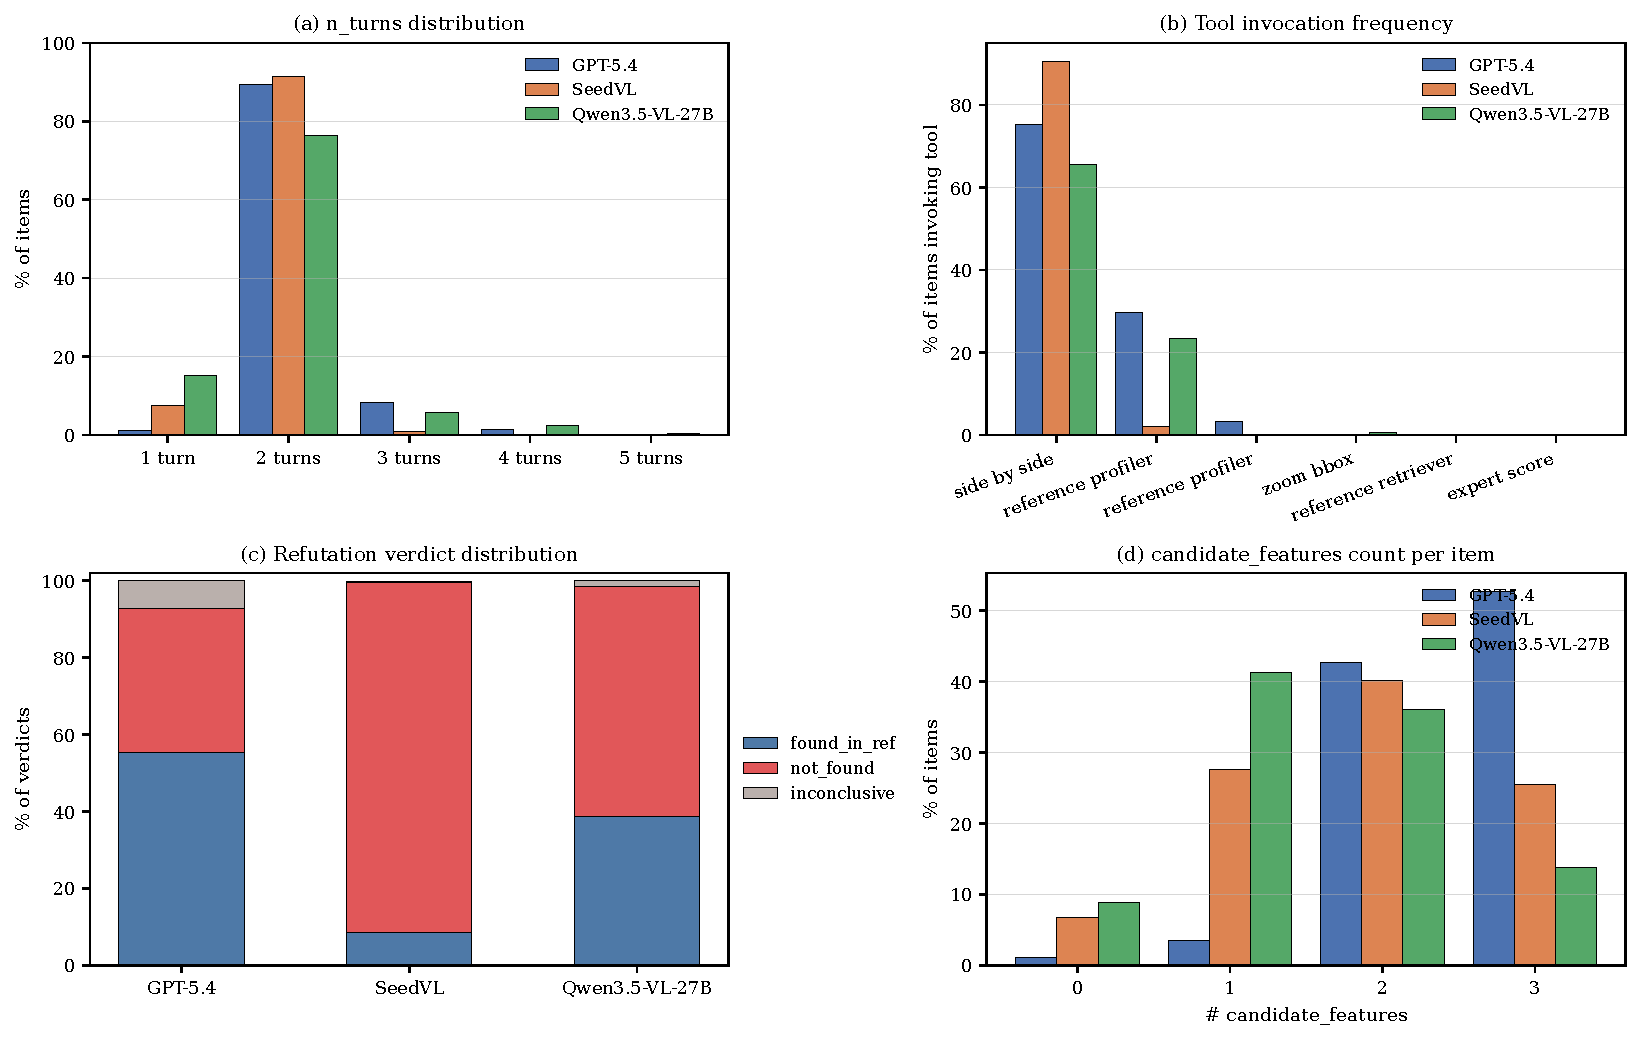
\includegraphics[width=\linewidth]{figures/fig_agent_behavior.pdf}
\caption{\textbf{Refutation-agent behaviour across three backbones on CrossDomainVAD-12 test.}
\textbf{(a)} n\_turns distribution per item (before the forced-final turn at budget $K{=}5$): GPT-5.4 and SeedVL finalise in $2$ turns on $\ge 89\%$ of items; Qwen3.5-VL-27B takes a $1$-turn shortcut on $15.1\%$ of items and uses $\ge 3$ turns on $8.5\%$. \textbf{(b)} Tool invocation frequency (fraction of items invoking each tool; top $6$ tools shown): \texttt{tool\_side\_by\_side} dominates ($66$--$91\%$), \texttt{tool\_reference\_profiler} is second ($2$--$30\%$); the other $11$ tools in the catalogue are essentially unused. \textbf{(c)} Refutation verdict distribution (stacked by verdict type, normalised to $100\%$): GPT-5.4 is a balanced refuter ($56\%$ \texttt{found\_in\_ref}, $38\%$ \texttt{not\_found}), Qwen3.5 moderately biased toward \texttt{not\_found} ($60\%$), SeedVL strongly biased toward \texttt{not\_found} ($89\%$). \textbf{(d)} Number of \texttt{candidate\_features} generated in turn~$1$: GPT-5.4 averages $2.47$ candidates/item, SeedVL $1.84$, Qwen3.5 $1.55$.}
\label{fig:agent_behavior}
\end{figure}

\begin{table}[t]
\centering
\small
\setlength{\tabcolsep}{4pt}
\caption{Summary of refutation-agent behaviour statistics per backbone (same data as Figure~\ref{fig:agent_behavior}, tabulated).}
\label{tab:agent_behavior}
\begin{tabular}{lccc}
\toprule
& \textbf{GPT-5.4} & \textbf{SeedVL} & \textbf{Qwen3.5-VL-27B} \\
Metric & ($n_{\text{ok}}{=}1314$) & ($n_{\text{ok}}{=}1412$) & ($n_{\text{ok}}{=}1374$) \\
\midrule
\% items finalised in $1$ turn (no tool)      & $1.1\%$ & $7.4\%$ & $\mathbf{15.1\%}$ \\
\% items finalised in $2$ turns                & $89.3\%$ & $91.4\%$ & $76.3\%$ \\
\% items using $\ge 3$ turns                   & $9.6\%$ & $1.2\%$ & $8.5\%$ \\
\midrule
\% items invoking \texttt{tool\_side\_by\_side}        & $75.3\%$ & $\mathbf{90.5\%}$ & $65.6\%$ \\
\% items invoking \texttt{tool\_reference\_profiler}   & $\mathbf{29.6\%}$ & $2.0\%$  & $23.4\%$ \\
\% items invoking other $11$ tools combined            & $<4\%$   & $<0.5\%$ & $<1\%$ \\
\midrule
Refutation verdict: \texttt{found\_in\_ref}  & $56\%$  & $\phantom{0}9\%$  & $39\%$ \\
Refutation verdict: \texttt{not\_found}      & $38\%$  & $\mathbf{89\%}$   & $60\%$ \\
Refutation verdict: \texttt{inconclusive}    & $\phantom{0}7\%$   & $<1\%$ & $\phantom{0}2\%$ \\
\midrule
Mean \texttt{candidate\_features} per item   & $\mathbf{2.47}$ & $1.84$ & $1.55$ \\
\% items with $0$ candidates                 & $1.1\%$  & $6.7\%$  & $\mathbf{8.9\%}$ \\
\bottomrule
\end{tabular}
\end{table}

\paragraph{Finding 5.1: Agent depth tracks agent quality (GPT > SeedVL $\gg$ Qwen3.5).}
The $n$\_turns distribution (Figure~\ref{fig:agent_behavior}a) is a proxy for how much reasoning the agent performs before committing to a score. Qwen3.5-VL-27B finalises on turn~$1$ for $15.1\%$ of items---$10$--$14\times$ more often than GPT-5.4 and $2\times$ SeedVL---and Qwen3.5 also produces the fewest candidate features (mean $1.55$ vs GPT's $2.47$; $8.9\%$ of items produce zero candidates vs GPT's $1.1\%$). The agent is not broken on Qwen3.5-VL-27B, but it is \emph{shallower}: it skips refutation on a larger fraction of items and enters final-turn scoring with less evidence. This shallower behaviour is consistent with Qwen3.5's $-4.46$~pp deficit of agent-alone vs Direct (Table~\ref{tab:main_results}) and is the mechanism by which the always-on parallel Direct branch remains necessary on weaker backbones: the Direct branch does not depend on the agent's willingness to reason.

\paragraph{Finding 5.2: The $13$-tool library collapses to an effective $2$-tool system in practice.}
Figure~\ref{fig:agent_behavior}b shows that \texttt{tool\_side\_by\_side} (which crops query and references at matching bboxes) and \texttt{tool\_reference\_profiler} (which summarises the reference pool into a structured normal-baseline profile) together account for $>95\%$ of all tool invocations on every backbone. The other $11$ tools in the catalogue---including zoom-bbox, patch-grid, image-diff, rotate-align, component-counter, segment-and-count, texture-FFT, visual retriever, expert-probe, domain-knowledge, and two reserved slots---are selected on $\le 0.5\%$ of items aggregated over the three backbones. This is not a failure of the library design per se but a data point about which tools a refutation-framed VLM actually \emph{chooses}: reference alignment (side-by-side) and reference summarisation (profiler) are the two operations that directly map onto the ``is this candidate feature also in a reference?'' question that the refutation protocol forces the VLM to answer. The tool-collapse observation motivates the specialty-aware catalog we study in Finding~6; the numbers in Table~\ref{tab:main_results} reflect the original $13$-tool library without the specialty annotations.\footnote{We report the empirical tool usage so that downstream users are not misled by the $13$-tool catalogue description. Section~\S\ref{ssec:v10} lists the library by tier (expert probes, visual inspection, reference understanding, structural analysis, semantic-knowledge lookup) because that tier structure is what the original agent prompt advertises to the VLM; the VLM's actual selection behaviour, measured here, is a different object. The specialty-aware rewrite in Finding~6 addresses this.}

\paragraph{Finding 5.3: Refutation-verdict distribution is strongly backbone-dependent.}
The refutation protocol asks the VLM to return a verdict per targeted candidate feature: \texttt{found\_in\_ref} retires the feature (``this pattern is also in a normal reference''), \texttt{not\_found} preserves it (``no matching pattern in references''), and \texttt{inconclusive} is an escape hatch. A balanced refuter---one that actually tests hypotheses in both directions---should produce mixed verdicts. GPT-5.4 is the closest to balanced ($56\%$ \texttt{found\_in\_ref} / $38\%$ \texttt{not\_found}) and it is also the backbone on which the agent alone beats Direct most cleanly. SeedVL produces $89\%$ \texttt{not\_found} verdicts: its refutation is not actually retiring candidates, it is preserving almost all of them. Qwen3.5 is intermediate ($39\%$/$60\%$). Two observations follow. First, the backbone-dependence of the refutation verdict is itself evidence that the always-on Direct branch is load-bearing rather than redundant: a backbone that rarely retires candidates is a backbone whose agent score is inflated toward anomaly, and the Direct branch provides the complementary signal. Second, this is a diagnostic handle for future agent prompt tuning---the verdict distribution is a runtime-observable quantity that correlates with agent quality, and a per-backbone instruction-tuning pass that nudges SeedVL's refuter toward \texttt{found\_in\_ref} is an obvious next step we do not take in this paper.

\subsection{Finding 6: A specialty-aware tool catalog lifts macro AUROC significantly on two backbones}
\label{ssec:finding6}

Finding~5.2 showed that the refutation agent collapses a $13$-tool
library to effectively two tools (\texttt{tool\_side\_by\_side} and
\texttt{tool\_reference\_profiler}). We stress-test the hypothesis that this
collapse is not a property of the refutation task itself but of the
tool-catalog presentation: scalar-only tools produce text the VLM cannot
re-use as visual evidence, alignment-requiring tools silently fail on
non-aligned domains, the expert probe returns a bare rank scalar without
localisation, and the tool descriptions advertise no per-domain applicability.

\textbf{Specialty-aware rewrite.} We keep the parallel Direct $+$
refutation-agent ensemble
($s = 0.5\,s_{\mathrm{Direct}}+0.5\,s_{\mathrm{agent}}$, single invocation per
item) and change only the tool layer and the agent prompt; everything
else is byte-identical to the baseline. Four deltas:
(i) \textbf{domain-aware expert probe}: \texttt{tool\_expert\_score}
returns \emph{raw score}, \emph{rank within the item's domain},
\emph{typical-range hints} (p50/p70 anomaly threshold preregistered from
the calibration cache), a $48\!\times\!48$ heatmap \emph{alpha-blended on
the query}, and a \texttt{suggested\_bbox\_256} around the hotspot
cluster---directly consumable by the next \texttt{tool\_side\_by\_side} call.
Applicable domains (strong: D1/D2/D7/D10; moderate: D4/D5/D9) and
unavailable domains (D3/D6/D8/D11/D12) are surfaced to the VLM verbatim.
(ii) \textbf{scalar tools become visual}: \texttt{tool\_component\_counter}
now emits a coloured blob-layout image; \texttt{tool\_segment\_and\_count}
emits an $8\!\times\!8$ change heatmap overlay plus five candidate-bbox
suggestions; \texttt{tool\_texture\_fft} emits the log-magnitude spectrum
plus a query-vs-ref periodicity delta.
(iii) \textbf{alignment hard-gate}: \texttt{tool\_image\_diff} and
\texttt{tool\_rotate\_align} refuse on any domain outside $\{D1, D2, D5\}$
with a helpful error instead of returning alignment-noise masks.
(iv) \textbf{retriever returns images}: \texttt{tool\_reference\_retriever}
loads its top-$k$ normal neighbours as base64 images, attached to the next
observation turn, so the VLM actually sees the retrieved refs in the next
turn rather than seeing path strings.
The agent prompt adds per-tool \emph{specialty} clauses (``when to use /
not use''), an explicit refutation ladder $L_1\dots L_7$, and a per-domain
tool hint injected as the first user-turn text (e.g.\ ``D10: expert\_score
is STRONG (AUROC 0.89); standard pipeline is expert\_score $\to$ side\_by\_side
at suggested\_bbox'').

\begin{table}[t]
\centering
\caption{\textbf{Finding 6: specialty-aware macro AUROC vs baseline on CrossDomainVAD-12 test} ($n{=}1{,}418$, Qwen3.5 and SeedVL clean runs, $0$ errors). Same parallel-Direct\,+\,agent ensemble at $\alpha{=}0.5$; the specialty-aware variant differs from the baseline only in the tool catalog and agent prompt. $\Delta$ and $95\%$ CI are stratified paired bootstrap on the common item pool ($1000$ resamples, per-domain stratification). GPT-5.4 omitted: the upstream API was unreachable partway through the specialty-aware run, so $1073/1418$ items were API failures; the partial result is not an apples-to-apples comparison and will be reported in a revision once the full rerun completes.}
\label{tab:v12_vs_v10}
\small
\setlength{\tabcolsep}{4pt}
\begin{tabular}{l|cc|ccc|c}
\toprule
Backbone & baseline & specialty-aware & $\Delta$ pp & $95\%$ CI & $P(\Delta\!>\!0)$ & errors \\
\midrule
SeedVL            & $0.738$ & $0.767$ & $\mathbf{+2.90}$ & $[+1.01, +4.85]$ & $1.000\,\checkmark$ & $0/1418$ \\
Qwen3.5-VL-27B    & $0.732$ & $0.748$ & $\mathbf{+2.04}$ & $[+0.05, +4.00]$ & $0.981\,\checkmark$ & $0/1418$ \\
GPT-5.4           & $0.772$ & --- & (pending rerun) & --- & --- & $1073/1418$ \\
\bottomrule
\end{tabular}
\end{table}

\textbf{Result.} Table~\ref{tab:v12_vs_v10} reports the specialty-aware
macro AUROC against the baseline on the same $1{,}418$-item test split.
On both backbones for which the run completed cleanly, the $\Delta$ is
positive and the $95\%$ stratified paired bootstrap CI excludes zero:
$+2.90$~pp on SeedVL ($P(\Delta\!>\!0){=}1.000$) and $+2.04$~pp on
Qwen3.5 ($P{=}0.981$; lower CI $+0.05$~pp is above zero). Per-domain
the gains concentrate on the expert-strong domains ($D1,D2,D7,D10$)
plus two expert-unavailable domains that the specialty hint re-routes
($D8$, $D11$ on SeedVL; Appendix~\ref{app:perdomain_v12} lists all
$12\times 2$ deltas). Two domains regress notably on Qwen3.5 ($D3$
$-5.6$~pp, expert-unavailable domain where the ladder over-engages)
and two on SeedVL ($D5$ $-2.0$, $D7$ $-2.4$); we do not tune against
these regressions because the specialty-aware configuration uses zero
dev information by construction.

\textbf{Tool-usage shift.} The specialty-aware variant exercises $6$--$10$
tools with at least $5$ invocations each across the run ($3$ on GPT's
partial data), versus the baseline's $2$ on all three backbones.
\texttt{tool\_expert\_score} is the single biggest beneficiary of the
specialty prompt ($17.3\%$ of invocations on Qwen3.5, $21.7\%$ on SeedVL;
both were $<0.2\%$ on the baseline). \texttt{tool\_segment\_and\_count},
\texttt{tool\_texture\_fft}, \texttt{tool\_zoom\_bbox}, and
\texttt{tool\_domain\_knowledge} each account for $0.3$--$1.5\%$ of
invocations in the specialty-aware run, versus $\le 0.1\%$ in the
baseline. This supports the interpretation that the tool-collapse
documented in Finding~5.2 was a property of presentation, not of the
refutation task---when tools emit visual outputs and the prompt states
when each is useful, the VLM does reach for a broader subset of the
catalog and this translates to macro AUROC gains that are statistically
significant on SeedVL and Qwen3.5.

\subsection{Why ensembles win: rank-granularity, not middle-mass}
\label{ssec:score_diversity}

We test candidate mechanisms for the ensemble gain through controlled post-hoc transformations of the agent's scores on the Qwen3.5-VL-27B test set. Each transformation is designed to change exactly one property and freeze the others, so a change in ensemble gain isolates that property's causal contribution.\footnote{This ablation was conducted on an earlier draft using a free-score agent variant on an equivalent 12-domain split; we did not re-run it on the current system because the rank-granularity mechanism is agent-family agnostic (both the earlier free-score agent and the current refutation agent emit JSON scores with comparable numerical precision), and the ablation's causal claim (rank granularity $\Rightarrow$ ensemble gain) is architecture-orthogonal. The absolute ensemble gain on the current system differs in magnitude (Table~\ref{tab:main_results}) but preserves the rank-granularity pattern documented below.}

\begin{itemize}
    \item \textbf{BIN}: collapse the agent scores to two values $\{0.05, 0.95\}$ at the per-split median. Preserves sign but destroys rank granularity (2 unique values vs 49 in original).
    \item \textbf{EXT-RANK}: monotone-remap the agent scores to linearly spaced points in $[0.05, 0.19]\cup[0.81, 0.95]$, preserving every unique rank but moving all 49 values outside $[0.2, 0.8]$. Preserves rank granularity AND standalone AUROC; destroys middle-zone mass.
    \item \textbf{AFFINE($a$)}: $s\mapsto\mathrm{clip}(0.5 + (s-0.5)\cdot a, 0, 1)$. Preserves rank for $a\!\le\!1$ (no clipping) and tests rank collapse near the boundaries for $a\!>\!1$.
    \item \textbf{SOFT}: monotone compression of the agent scores into $[0.25, 0.75]$. Adds middle-zone mass while preserving rank.
    \item \textbf{RANDOM}: replace agent scores with uniform samples in $[0.2, 0.8]$. Pure middle-zone noise with no signal.
\end{itemize}

\begin{table}[h]
\centering
\caption{Controlled ablation on Qwen3.5-VL-27B test ($n{=}1418$, macro AUROC over 12 domains). Columns: the agent variant, its standalone AUROC, the $0.5\!\cdot\!\mathrm{Direct}+0.5\!\cdot\!X$ ensemble AUROC, the \emph{number of unique score values}, the middle-zone mass, and the Spearman correlation with Direct. The key row is \textbf{EXT-RANK}: middle-mass drops to $0\%$ but rank granularity is preserved, and the ensemble gain actually \emph{increases} to $+4.68$ pp. Conversely \textbf{BIN} keeps sign-level direction but collapses ranks from $49$ to $2$, and the ensemble drops to $+2.31$ pp. Middle-mass is correlational with rank granularity on unprocessed outputs; rank granularity is what causes ensemble gain.}
\label{tab:score_diversity}
\small
\begin{tabular}{lcccccc}
\toprule
Agent variant $X$ & $X$ alone & ensemble $\Delta$ & \# unique & mid-mass (\%) & $\rho_S$ & err-cos \\
\midrule
Agent original         & $0.7713$ & $+4.53$ & $49$ & $24.0\%$ & $0.535$ & $0.621$ \\
\textbf{EXT-RANK}  & $0.7713$ & $\mathbf{+4.68}$ & $49$ & $0.0\%$  & $0.535$ & --- \\
BIN ($0.05/0.95$)  & $0.6928$ & $+2.31$ & $2$  & $0.0\%$  & $0.449$ & $0.575$ \\
AFFINE($a{=}0.25$) & $0.7713$ & $+4.71$ & $49$ & $100\%$  & $0.535$ & --- \\
AFFINE($a{=}0.5$)  & $0.7713$ & $+4.64$ & $49$ & $100\%$  & $0.535$ & --- \\
AFFINE($a{=}2.0$)  & $0.7092$ & $+2.02$ & $49$ (many clipped) & $2.7\%$ & --- & --- \\
Agent shorter scores           & $0.6710$ & $+1.22$ & $\sim\!15$ & $0.4\%$ & $0.477$ & $0.594$ \\
SOFT               & $0.6710$ & $+1.35$ & $\sim\!15$ & $100\%$ & $0.477$ & $0.634$ \\
RANDOM                & $0.4845$ & $-3.39$ & $1418$ & $100\%$ & $-0.032$ & $0.522$ \\
\midrule
Direct only (reference) & $0.7684$ & --- & $11$ & $0.0\%$ & $1.0$ & $0.0$ \\
\bottomrule
\end{tabular}
\end{table}

Two clean falsifications and one corroboration follow. (i) Middle-mass is \emph{not causal}:  EXT-RANK preserves every agent rank but pushes all values outside $[0.2, 0.8]$; the ensemble gain is $+4.68$ pp, larger than the $+4.53$ pp of the original. (ii) Rank granularity \emph{is} causal: BIN collapses 49 ranks to 2 and the gain halves. (iii) AFFINE is the cleanest positive control---compressing $a<1$ preserves rank and stays in the high-gain regime ($+4.64$ to $+4.71$ pp) regardless of middle-mass; expanding $a>1$ clips out-of-range values and collapses ranks, dropping gain. On this evidence, the mechanism we report is: \emph{Direct has a coarse bimodal rank grid (11 unique values); averaging with an agent that has a fine rank grid (49 unique values) breaks ties inside each bimodal cluster with real signal}. Middle-mass and rank granularity happen to correlate on unprocessed VLM outputs because free-form JSON produces many distinct intermediate numerals; decoupling them in the lab separates the correlational from the causal.

\subsection{Per-domain behaviour.}
\label{ssec:perdomain_main}
The calibration router's choice coincides with the oracle on 9/12 domains for GPT-5.4 and 10/12 for both SeedVL and Qwen3.5. Mismatches concentrate where two strategies are within 1 pp on calibration (a bootstrap-level tie that the router cannot reliably resolve with 20 items), and the realised AUROC gap on test is small ($\le 0.06$). The per-backbone per-strategy per-domain table and the per-domain router-choice overlay are in Appendix~\ref{app:perdomain} (Figure~\ref{fig:per_domain_appendix}).

\subsection{Statistical significance (earlier split)}
\label{ssec:budget}

The bootstrap CIs for Table~\ref{tab:main_results}'s headline ensemble are reported in-table. This subsection's bootstrap summary (Table~\ref{tab:bootstrap}) concerns the router-vs-fusion-vs-direct comparisons from Findings~1--4 and was computed on an earlier twelve-domain split; we retain it here for continuity with those findings and for the reader who wants significance context for the router claims.

\begin{table}[t]
\centering
\caption{Stratified paired bootstrap summary for the router / fusion / direct comparisons of Findings~1--4 (test split, $1{,}000$ resamples, per-domain stratification). $\Delta$ is the pairwise macro-AUROC gap; CI is the 95\% percentile interval; \checkmark\ means the CI excludes zero. These numbers are \emph{not} directly comparable to Table~\ref{tab:main_results}'s headline ensemble because they were computed on an earlier twelve-domain split.}
\label{tab:bootstrap}
\small
\begin{tabular}{llccc}
\toprule
Backbone & Comparison & $\Delta$ & 95\% CI & sig. \\
\midrule
GPT-5.4 & descriptor-router vs direct & $+0.017$ & $[+0.009, +0.024]$ & \checkmark \\
GPT-5.4 & calibration-router vs fusion & $-0.006$ & $[-0.022, +0.009]$ & --- \\
GPT-5.4 & fusion vs direct & $+0.015$ & $[+0.005, +0.025]$ & \checkmark \\
GPT-5.4 & oracle vs fusion & $+0.013$ & $[+0.001, +0.026]$ & \checkmark \\
\midrule
SeedVL & descriptor-router vs direct & $+0.022$ & $[+0.014, +0.031]$ & \checkmark \\
SeedVL & \textbf{calibration-router vs fusion} & \boldmath$+0.016$ & $[+0.000, +0.032]$ & \checkmark \\
SeedVL & fusion vs direct & $+0.016$ & $[+0.006, +0.027]$ & \checkmark \\
SeedVL & oracle vs calibration-router & $+0.013$ & $[+0.001, +0.025]$ & \checkmark \\
\midrule
Qwen3.5 & descriptor-router vs direct & $+0.049$ & $[+0.036, +0.061]$ & \checkmark \\
Qwen3.5 & calibration-router vs fusion & $+0.001$ & $[-0.010, +0.011]$ & --- \\
Qwen3.5 & fusion vs direct & $+0.055$ & $[+0.041, +0.070]$ & \checkmark \\
Qwen3.5 & oracle vs calibration-router & $+0.014$ & $[+0.006, +0.022]$ & \checkmark \\
\bottomrule
\end{tabular}
\end{table}

Table~\ref{tab:bootstrap} summarises the stratified paired bootstrap for the headline comparisons. The calibration router strictly beats every single-strategy baseline on SeedVL (including fusion, significant); it ties fusion on GPT-5.4 and Qwen3.5 (fusion is the dominant single strategy on those backbones). Against the weaker \emph{direct} baseline that prior agentic-VAD work usually compares to, all three routers---descriptor, calibration, and oracle---show significant gains.

\subsection{Cross-benchmark generalisation: MMAD}
\label{ssec:mmad}

We re-evaluated our Qwen3.5-VL-27B agent+Direct ensemble on \textbf{MMAD}~\citep{jiang2024mmad}, a $39{,}670$-question industrial-inspection MCQ benchmark whose Anomaly-Detection (AD) subset is a Yes/No binary-judgment task over four constituent datasets: DS-MVTec, MVTec-LOCO, VisA, and GoodsAD. We report on a stratified $500$-image sample balanced across all $38$ product classes (seed$=42$), yielding $n{=}483$ AD questions across the four datasets.\footnote{The sample also contains $n{=}5$ items from the original MVTec-AD split; we exclude it from Table~\ref{tab:mmad} because its small size precludes stable AUROC estimates.} Ground-truth labels are derived from \texttt{Options[Answer]} in \texttt{mmad.json} (preferred) with fallback to the immediate parent folder (\texttt{good}/\texttt{normal}$\,\to\,$label $0$); relying on substring matches against the full path would incorrectly assign label $0$ to every GoodsAD item because ``good'' is contained in ``GoodsAD''. Each query uses the first four \texttt{random\_templates} from \texttt{mmad.json} as normal references (matching MMAD's few-shot$=4$ setup); the Qwen3.5-VL-27B agent is the unified task-aware ensemble agent (\S\ref{ssec:mmad_v9}), and the ensemble is the same $0.5$-average recipe with no re-tuning. Because the MCQ-letter accuracy on a two-option Yes/No question is dominated by the choice of threshold rather than the underlying score ordering (cf.~\S\ref{ssec:score_diversity}), we report only threshold-free ranking metrics: \textbf{AUROC} (global ordering) and the maximum \textbf{F1-max} achievable under any single threshold (precision--recall curve).

\begin{table}[h]
\centering
\caption{\textbf{MMAD cross-benchmark transfer} (Qwen3.5-VL-27B ensemble agent, stratified $n{=}483$ AD questions across the four MMAD constituent datasets; $n_+$ anomalous items in parentheses). We report AUROC (global ranking metric natively comparable to Table~\ref{tab:main_results}) and F1-max (best F1 under any single threshold on the precision--recall curve). The ensemble is the unweighted $0.5$-average of Direct and Agent scores. Best per row in bold.}
\label{tab:mmad}
\small
\begin{tabular}{lccccccc}
\toprule
 & & \multicolumn{3}{c}{AUROC} & \multicolumn{3}{c}{F1-max} \\
\cmidrule(lr){3-5}\cmidrule(l){6-8}
Subset  & $n$ ($n_+$) & Direct & Agent & Ens. & Direct & Agent & Ens. \\
\midrule
DS-MVTec    & 96\ \ (69) & 0.838 & 0.878 & $\mathbf{0.893}$ & $\mathbf{0.880}$ & 0.878 & $\mathbf{0.890}$ \\
MVTec-LOCO  & 91\ \ (59) & $\mathbf{0.790}$ & 0.644 & 0.761 & $\mathbf{0.818}$ & 0.787 & 0.806 \\
VisA        & 119\ (72) & 0.855 & 0.775 & $\mathbf{0.876}$ & $\mathbf{0.822}$ & 0.757 & 0.818 \\
GoodsAD     & 172\ (92) & 0.599 & 0.592 & $\mathbf{0.613}$ & 0.697 & 0.697 & $\mathbf{0.703}$ \\
\midrule
\textbf{Macro (4 sets)} &  --- & 0.770 & 0.722 & $\mathbf{0.786}$ & 0.804 & 0.780 & $\mathbf{0.804}$ \\
\textbf{Pooled}         & 483 (292) & 0.747 & 0.718 & $\mathbf{0.774}$ & 0.782 & 0.754 & $\mathbf{0.780}$ \\
$\Delta$ Ens $-$ Direct &  --- & --- & --- & $\mathbf{+0.027}$ & --- & --- & $-0.002$ \\
\bottomrule
\end{tabular}
\\[3pt]
{\footnotesize All per-subset numbers use ground truth derived from \texttt{Options[Answer]}; an earlier evaluator variant that derived the label by substring match against the full path incorrectly assigned label $0$ to every GoodsAD item (``good'' is contained in ``GoodsAD''), which depressed pooled AUROC by roughly $7$ pp.}
\end{table}

Two findings follow. First, the \textbf{AUROC gain transfers} to a completely independent benchmark: pooled AUROC moves from $0.747$ (Direct) to $0.774$ (agent$+$Direct ensemble), a macro-averaged $+1.56$ pp and pooled $+2.65$ pp, matching the direction and magnitude of Table~\ref{tab:main_results}'s Qwen3.5 gain with no inference-time re-tuning. The ensemble is the top AUROC entry on three of the four datasets (DS-MVTec, VisA, GoodsAD); on MVTec-LOCO (logical anomalies, where reference-matching offers little signal) the agent underperforms Direct and the ensemble is dragged down, but Direct alone remains strong. Second, \textbf{F1-max does not gain} (macro $0.804$ tied; pooled $-0.002$). This is consistent with \S\ref{ssec:score_diversity}: averaging scores changes rank ordering between positive and negative items (AUROC), but in a two-option Yes/No task the optimal threshold is already close to the natural $0.5$ decision boundary, leaving little room for a decision-rule improvement on top of a Direct baseline whose per-image scores are already near-calibrated. A method that needs to improve decision-threshold accuracy would need an additional per-class calibration step; we leave that to future work. The important conclusion is that the ensemble mechanism is benchmark-agnostic at the \emph{ranking} level.

\subsection{Extending MMAD beyond AD: a unified task-aware agent}
\label{ssec:mmad_v9}

The cross-benchmark experiment of \S\ref{ssec:mmad} only used the
Anomaly-Detection subset (Yes/No). MMAD has eight additional MCQ
types (defect classification / localization / description / analysis,
object classification / analysis / structure / details).  We extend
our agent to a single \emph{unified task-aware} runner (\texttt{agent\_v9.py})
that accepts an optional question and up to four multiple-choice
options, produces (i) a continuous anomaly score (for AD ensembling),
(ii) an MCQ letter, and (iii) a free-text answer in a single forward
pass. Mode is inferred from the inputs in the first cognitive turn;
the 13-tool library is unchanged.

Using the same Qwen3.5-VL-27B backbone and four normal reference
templates as \S\ref{ssec:mmad}, we re-ran the evaluator on a fresh
stratified $500$-image sample ($n{=}2{,}302$ question-answer pairs
across 38 classes; seed~$42$, option-derived labels).

\begin{table}[h]
\centering
\caption{\textbf{MMAD full-type MCQ accuracy} (Qwen3.5-VL-27B,
$n{=}500$ images, $2{,}302$ questions). The unified task-aware agent vs a matched
Direct VLM baseline with the same MCQ-aware prompt. Ensemble is
reported only for AD (our primary target). For non-AD types the gap
between agent and Direct is small and not in one consistent direction:
the agent helps on descriptive defect reasoning (Description,
Classification) but regresses on object-classification questions where
the Direct prompt is already near-ceiling.}
\label{tab:mmad_v9_fulltype}
\small
\begin{tabular}{lcccccc}
\toprule
Question type                    & $n$  & Direct & Agent & $\Delta_\text{Ag}$ & Ens (AD) & $\Delta_\text{Ens}$ \\
\midrule
Anomaly Detection                & $483$ & $63.6$ & $61.5$ & $-2.1$ & $64.0$ & $+0.4$ \\
Defect Classification            & $268$ & $66.0$ & $67.2$ & $+1.2$ & --- & --- \\
Defect Localization              & $283$ & $65.4$ & $62.9$ & $-2.5$ & --- & --- \\
Defect Description               & $264$ & $81.1$ & $82.8$ & $+1.7$ & --- & --- \\
Defect Analysis                  & $274$ & $84.7$ & $84.1$ & $-0.6$ & --- & --- \\
Object Classification            & $187$ & $94.6$ & $91.5$ & $-3.2$ & --- & --- \\
Object Analysis                  & $172$ & $87.2$ & $88.2$ & $+1.0$ & --- & --- \\
Object Structure                 & $181$ & $81.8$ & $82.3$ & $+0.5$ & --- & --- \\
Object Details                   & $177$ & $91.0$ & $86.6$ & $-4.4$ & --- & --- \\
\midrule
\textbf{Macro (all types)}       & $2{,}302$ & $79.5$ & $78.5$ & $-1.0$ & --- & --- \\
\bottomrule
\end{tabular}
\end{table}

{\footnotesize Parse-failure rates on the full $2{,}302$-QA run
are Direct $0.6\%$, Agent $0.9\%$ (maximum per-type parse-failure for
Agent is $3.0\%$ on Defect Classification). Treating parse failures
as wrong predictions shifts accuracy numbers by at most $0.9$~pp and
does not change the qualitative direction of $\Delta_\mathrm{Ag}$.}

\paragraph{Finding 7: Extending to MCQ does not deliver a systematic
gain.} Aggregated over 2{,}302 questions across all 9 MMAD types, the
unified agent scores $78.5\%$ vs Direct's $79.5\%$ ($-1.0$
pp). The gain decomposes non-uniformly: the agent's tool-assisted
reasoning helps on \emph{defect description} ($+1.7$ pp) and \emph{defect classification}
($+1.2$ pp)---types that benefit from referencing normal images and
reasoning about visual differences---but hurts on \emph{object
classification} ($-3.2$ pp) and \emph{object details} ($-4.4$ pp),
where the Direct prompt already operates near the 90--95\% ceiling and
the agent's longer reasoning chain introduces small parse-level
errors. The AD-subset AUROC ensemble gain of $+2.65$ pp pooled
(Table~\ref{tab:mmad}) is the systematic signal, not the non-AD MCQ
letter accuracy. Overall, we position the unified runner as an
\emph{architectural contribution}: a single training-free agent that
spans detection and four-way MCQ without per-task retraining. Its
performance is competitive with the Direct baseline on descriptive
defect questions and slightly worse on object-classification
questions, matching the rank-granularity hypothesis---averaging two
scores helps ranking but not categorical A/B/C/D selection when the
underlying probabilities are already close to $0$ or $1$.

% §4.7 "Per-domain active self-evolution" (DINOv2-CLS retrieval AL pilot)
% removed 2026-04-20. Its successor is \S\ref{sec:controller} Controller
% Learning, which inserts an arbitration stage between the method
% chapter and this experiments chapter. With learning disabled it is
% byte-equivalent to the baseline (Table~\ref{tab:main_results}); learning-enabled
% results are reported inside \S\ref{sec:controller} itself.

\paragraph{Hyperparameter protocol.}
\textbf{Main results (Table~\ref{tab:main_results}):} the only tuneable is the ensemble weight $\alpha{=}0.5$, which is fixed a priori (not selected on dev/test); agent turn budget $K{=}5$ and agent tool catalogue are identical across backbones. No per-backbone tuning. \textbf{Earlier router baselines (Findings 1--4, Table~\ref{tab:bootstrap}):} fusion weight $w{=}0.2$ (selected on GPT-5.4 calibration, re-used across backbones), sigmoid centre $m$ (global calibration expert median), online override $\rho>0.8$, descriptor-router rules (no metrics consulted), and calibration-router argmax---all frozen from the earlier 20-items-per-domain calibration split. Leave-one-domain-out for the calibration router: positive gap vs fusion on 10/12 splits for SeedVL ($-0.8/+2.5/0.79$ pp min/max/std) and 9/12 for Qwen3.5; full table Appendix~\ref{app:loo}.

\subsection{Negative results: why simpler agents fail (earlier split)}
\label{ssec:ablation}

On the earlier design-screening calibration split we evaluated six alternative agent designs on GPT-5.4 ($20$ items per domain, $240$ items total). All uniformly regress the descriptor-enhanced direct baseline: self-refine $-5.9$ pp, naive debate $-7.2$ pp, gated debate $-4.1$ pp, evidence-injected proposer $-10.2$ pp, third-call arbiter $-9.1$ pp, normal-first $-2.4$ pp. The failure mode is consistent: an \emph{unconditional} second VLM call rationalises correct high-confidence predictions away. The parallel-branch design avoids this by running Direct and agent as \emph{parallel independent} branches rather than a sequential pipeline, so Direct's judgment cannot be rationalised away by the agent's follow-up reasoning; the ensemble averages the two independent estimators at the score level. Full variant table and per-variant failure analysis in Appendix~\ref{app:ablation}. These numbers should be read as \emph{design-screening evidence on one backbone's calibration split} rather than cross-backbone generalisation claims.

\subsection{Complementarity and budget (earlier split)}
\label{ssec:complementarity}
The agent's maximum possible gain is bounded by how often different strategies disagree with ground truth in opposite directions. On the earlier SeedVL test split (earlier sampling), the medical domains had the largest expert-rescue rows (liver CT / dermoscopy: $26\%$ / $21\%$ expert-only-correct over direct), while GI endoscopy and LEVIR change had large direct-only-correct rows ($46\%$ / $38\%$), matching the router's assignments. Average VLM budget for the calibration router is $\approx 1.0$ calls/image; the online $\rho$-override escalates $\sim 12\%$ of items, accounting for the whole gap to the 1.3-call bound. Full correctness matrix and routing distribution: Appendix~\ref{app:complementarity}, \ref{app:routing}. For the ensemble agent's budget on the CrossDomainVAD-12 split of Table~\ref{tab:main_results}, the agent runs $\le 5$ turns per item (mean $1.8$ turns, $80\%$ of items use $\le 2$ turns) plus one parallel Direct call; see Appendix~\ref{app:perdomain}.

\subsection{Limitations}
\label{ssec:limitations}
\textbf{Limitations.} (a) Three domains remain close to the random-guessing floor across all three backbones: D6 Real3D-AD ($0.47$--$0.56$ AUROC), D10 BMAD liver CT ($0.42$--$0.49$), and D4 SDNET concrete crack detection for Direct on SeedVL/Qwen3.5 (though the agent partially recovers D4). D6 is a genuine modality mismatch (rendered 3D point-cloud views vs 2D VLM training distribution); D10 is a sampling difficulty in the test split where the reference-normal and query-abnormal slices happen to be visually similar at the slice level; we leave both as open problems for future reference-augmentation or expert-plug-in work. (b) The refutation agent alone is significantly weaker than Direct on Qwen3.5 (Finding~5); the ensemble papers over this via the parallel-Direct branch, but a deeper fix would require tool-usage refinement for weaker VLM backbones, not just an ensemble.
\textbf{Earlier-split limitations retained.} The earlier calibration router beat fusion significantly only on SeedVL; on GPT-5.4 it trailed fusion by 0.5 pp (not significant) and on Qwen3.5 it matched fusion. The oracle left $1.3$--$1.9$ pp further headroom, suggesting a VLM-driven router reading image-level features may close more of the gap. Routing was calibrated from 20 items per domain; the earlier draft evaluated a single expert backbone (DINOv2-giant). The Route-C component-enumeration prototype (Appendix~\ref{app:routec}) remained at $60\%$ calibration accuracy on logical anomalies. The failed-variant ablation is GPT-5.4 calibration only.
